% \fs and \fmax must be defined before calling this picture.
\def\fs{10}
\def\fmax{5}
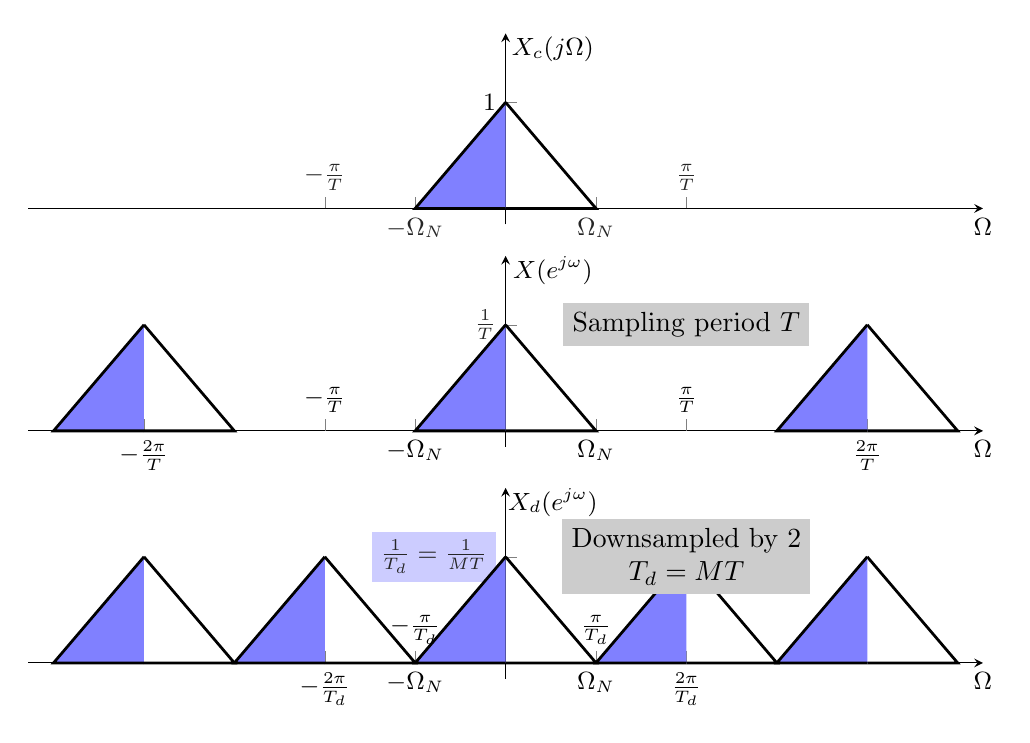
\begin{tikzpicture}
\onslide<1-|handout:1>{
\begin{axis}[
	name=plot1,
	axis lines*=middle,
	enlargelimits = true,
	clip=false,
	scale only axis,
	width=\textwidth,
	height=0.2\textwidth,
	ymin=0,
	ymax=3,
	xmin=-\fs-1,
	xmax=\fs+1,
	axis line style={->,>=stealth},
	xlabel={\small $\Omega$},
	ylabel={\small $X_c(j\Omega)$},
	every axis x label/.style={
		at={(ticklabel* cs:1)},
		%xshift=0.2cm,
		anchor=north,
	},
	every axis y label/.style={
		at={(ticklabel* cs:0.8)},
		anchor=south,
		xshift=0.6cm,
	},
	ytick=2,
	xtick=\empty,
	yticklabel={\small 1},
	xtick={-2.5, 2.5},
	xticklabels={\small $-\Omega_N$, \small $\Omega_N$},
	extra x ticks={-\fmax, \fmax},
	extra x tick labels={\small $-\frac{\pi}{T}$, \small $\frac{\pi}{T}$},
	extra x tick style={
		xticklabel style={yshift=0.7ex, anchor=south}
	},
	every outer y axis line/.append style={white!15!black},
	every x tick label/.append style={font=\color{white!15!black}},
	legend style={draw=white!15!black,fill=white,legend cell align=left}]
	\addplot[solid, line width=1pt] coordinates {(0, 2) (2.5, 0) (0, 0)};
	\addplot[solid, line width=1pt, fill=blue!50] coordinates {(0, 2) (-2.5, 0) (0, 0)};
\end{axis}
}
\onslide<2-|handout:1>{
\begin{axis}[
	name=plot2,
	at=(plot1.below south east), anchor=above north east,
	axis lines*=middle,
	enlargelimits = true,
	clip=true,
	scale only axis,
	width=\textwidth,
	height=0.2\textwidth,
	ymin=0,
	ymax=3,
	xmin=-\fs-1,
	xmax=\fs+1,
	axis line style={->,>=stealth},
	xlabel={\small $\Omega$},
	ylabel={\small $X(e^{j\omega})$},
	every axis x label/.style={
		at={(ticklabel* cs:1)},
		%xshift=0.2cm,
		anchor=north,
	},
	every axis y label/.style={
		at={(ticklabel* cs:0.8)},
		anchor=south,
		xshift=0.6cm,
	},
	xtick=\empty,
	ytick=2,
	yticklabels={\small $\frac{1}{T}$},
	xtick={-\fs, -2.5, 2.5, \fs},
	xticklabels={\small $-\frac{2\pi}{T}$, \small $-\Omega_N$, \small $\Omega_N$, \small $\frac{2\pi}{T}$},
	extra x ticks={-\fmax, \fmax},
	extra x tick labels={\small $-\frac{\pi}{T}$, \small $\frac{\pi}{T}$},
	extra x tick style={
		xticklabel style={yshift=0.7ex, anchor=south}
	},
	every outer y axis line/.append style={white!15!black},
	every y tick label/.append style={font=\color{white!15!black}},
	legend style={draw=white!15!black,fill=white,legend cell align=left}]
	\addplot[solid, line width=1pt] coordinates {(0, 2) (2.5, 0) (0, 0)};
	\addplot[solid, line width=1pt, fill=blue!50] coordinates {(0, 2) (-2.5, 0) (0, 0)};
	\addplot[solid, line width=1pt] coordinates {(\fs, 2) (\fs+2.5, 0) (\fs, 0)};
	\addplot[solid, line width=1pt, fill=blue!50] coordinates {(\fs, 2) (\fs-2.5, 0) (\fs, 0)};
	\addplot[solid, line width=1pt] coordinates {(-\fs, 2) (-\fs+2.5, 0) (-\fs, 0)};
	\addplot[solid, line width=1pt, fill=blue!50] coordinates {(-\fs, 2) (-\fs-2.5, 0) (-\fs, 0)};
	\addplot[solid, line width=1pt] coordinates {(-2*\fs, 2) (-2*\fs+2.5, 0) (-2*\fs, 0)};
	\addplot[solid, line width=1pt, fill=blue!50] coordinates {(-2*\fs, 2) (-2*\fs-2.5, 0) (-2*\fs, 0)};]
	\addplot[solid, line width=1pt] coordinates {(2*\fs, 2) (2*\fs+2.5, 0) (2*\fs, 0)};
	\addplot[solid, line width=1pt, fill=blue!50] coordinates {(2*\fs, 2) (2*\fs-2.5, 0) (2*\fs, 0)};
	\node[scale=1, fill=black!20] at (axis cs: 5, 2) {Sampling period $T$};
\end{axis}
}
\onslide<3|handout:1>{
\def\fsM{5}
\def\fmaxM{2.5} % 
\def\BWM{2.5} % WN * T_d = WN * 2 * T = 2 * (BW)
\begin{axis}[
	name=plot3,
	at=(plot2.below south east), anchor=above north east,
	axis lines*=middle,
	enlargelimits = true,
	clip=true,
	scale only axis,
	width=\textwidth,
	height=0.2\textwidth,
	ymin=0,
	ymax=3,
	xmin=-\fs-1,
	xmax=\fs+1,
	axis line style={->,>=stealth},
	xlabel={\small $\Omega$},
	ylabel={\small $X_d(e^{j\omega})$},
	every axis x label/.style={
		at={(ticklabel* cs:1)},
		%xshift=0.2cm,
		anchor=north,
	},
	every axis y label/.style={
		at={(ticklabel* cs:0.8)},
		anchor=south,
		xshift=0.6cm,
	},
	xtick=\empty,
	ytick=2,
	yticklabels={\small \tikz[baseline]{\node[fill=blue!20,anchor=base] {$\frac{1}{T_d} = \frac{1}{MT}$};}},
	xtick={-\fsM, -\BWM, \BWM, \fsM},
	xticklabels={\small $-\frac{2\pi}{T_d}$, \small $-\Omega_N$, \small $\Omega_N$, \small $\frac{2\pi}{T_d}$},
	extra x ticks={-\fmaxM, \fmaxM},
	extra x tick labels={\small $-\frac{\pi}{T_d}$, \small $\frac{\pi}{T_d}$},
	extra x tick style={
		xticklabel style={yshift=0.7ex, anchor=south}
	},
	every outer y axis line/.append style={white!15!black},
	every y tick label/.append style={font=\color{white!15!black}},
	legend style={draw=white!15!black,fill=white,legend cell align=left}]
	\addplot[solid, line width=1pt] coordinates {(0, 2) (\BWM, 0) (0, 0)};
	\addplot[solid, line width=1pt, fill=blue!50] coordinates {(0, 2) (-\BWM, 0) (0, 0)};
	\addplot[solid, line width=1pt] coordinates {(\fsM, 2) (\fsM+\BWM, 0) (\fsM, 0)};
	\addplot[solid, line width=1pt, fill=blue!50] coordinates {(\fsM, 2) (\fsM-\BWM, 0) (\fsM, 0)};
	\addplot[solid, line width=1pt] coordinates {(-\fsM, 2) (-\fsM+\BWM, 0) (-\fsM, 0)};
	\addplot[solid, line width=1pt, fill=blue!50] coordinates {(-\fsM, 2) (-\fsM-\BWM, 0) (-\fsM, 0)};
	\addplot[solid, line width=1pt] coordinates {(-2*\fsM, 2) (-2*\fsM+\BWM, 0) (-2*\fsM, 0)};
	\addplot[solid, line width=1pt, fill=blue!50] coordinates {(-2*\fsM, 2) (-2*\fsM-\BWM, 0) (-2*\fsM, 0)};]
	\addplot[solid, line width=1pt] coordinates {(2*\fsM, 2) (2*\fsM+\BWM, 0) (2*\fsM, 0)};
	\addplot[solid, line width=1pt, fill=blue!50] coordinates {(2*\fsM, 2) (2*\fsM-\BWM, 0) (2*\fsM, 0)};
	\node[scale=1, fill=black!20, align=center] at (axis cs: 5, 2) {Downsampled by 2 \\ $T_d = MT$};
\end{axis}
}
\end{tikzpicture}
